
\chapter{闭波导逆时偏移算法讨论}
\label{chapter:ref3}
在本章,我们主要讨论了平板声波闭波导模型下的逆时偏移算法。特别地,我们仅关注于在较为简单的闭波导模型,是否也会出现类似于第三章开波导模型逆时偏移算法所引出的问题\ref{pro_fatal}。通过分析和测试,我们将看到答案是肯定的。首先,我们列出平板声波闭波导两种边界的格林函数,其计算方法类似于之前推导开波导的格林函数,这方面的内容可以参考文献\cite{ch_cw,Xu1990The,Arens2011Direct}。然后我们在文献\cite{ch_cw}中闭波导逆时偏移算法的基础上,研究一种更有意思的点扩散函数,其与第三章的开波导点扩散函数是相互对应的。
\section{平板声波闭波导格林函数}
\subsection{Neumann格林函数}
令$N_w(x,y)$为对应于第一章所介绍的平板声波闭波导模型\ref{cwg}的格林函数,其满足如下方程:
\begin{eqnarray}\label{cwg_neumann}
\left\{
\begin{array}{lll}
\Delta_xN_w(x,y)+k^2N_w(x,y)=-\delta_y(x),&in& \R^2_h\\
& &\\
N_w(x,y)=0, &on&\Gamma_0\\
& &\\
\frac{\partial N(x,y)}{\partial x_2}=0, &on&\Gamma_h.
\end{array}
\right.
\end{eqnarray}
其中$\R^2_h=\{(x_1,x_2);x_1\in \R, x_2\in(0,h)\}$, $ \Gamma_0=\{(x_1,x_2);x_1\in \R, x_2=0\}$。利用格林函数$N_w(x,y)$为向外传播的解,直接计算可得:
\begin{equation}\label{f_Nw}
 N_w(x,y)=\frac{1}{2\pi}\int_{SIP}\hat N_w^y(\xi,x_2)e^{\i|x_1-y_1|\xi}d\xi
\end{equation}
其中Fourier变换$\hat N_w^y(\xi,x_2)$的表达式为:
\begin{equation}
\hat N_w^y(\xi,x_2)=\frac{\i}{2\mu}\left[e^{\i\mu|x_2-y_2|}-e^{\i\mu(x_2+y_2)}-\frac{2e^{\i\mu h}}{\cos(\mu h)}\sin(\mu x_2)\sin(\mu y_2)\right]
\end{equation}
然后通过留数定理,直接计算可得其波导模式展开表达式:
\begin{lemma}\label{mode_Nw}
设 $k\neq\frac{2n-1}{2h}\pi, n=1,2,\ldots$,则$N_w(x,y)$的波导模式展开表达式为:	
\begin{equation}
	N_w(x,y)=\sum\limits_{n=1}^{+\infty}\frac{\i}{h\xi_n}\sin(\mu_nx_2)\sin(\mu_ny_2)e^{\i\xi_n|x_1-y_1|}
\end{equation}
其中$\mu_n=\frac{2n-1}{2h}\pi, \xi_n=\sqrt{k^2-\mu_n^2}, n=1,2,\ldots$。 
\end{lemma}
\begin{remark}
 由引理\ref{mode_Nw}可知,存在正整数$\hat M>0$使得:当$n\leq\hat M$时,$\xi_n$为正实数;当$n>\hat M$时,$\xi_n$为虚部大于0的纯虚数。于是可对$N_w(x,y)$做如下分解:
 \begin{equation}
  N_w(x,y) = N_w^g(x,y)+N_w^{rad}(x,y)
 \end{equation}
其中
\begin{eqnarray}
\left\{
\begin{array}{lll}
 N_w^g(x,y)&=&\sum\limits_{n=1}^{\hat M}\frac{\i}{h\xi_n}\sin(\mu_nx_2)\sin(\mu_ny_2)e^{\i\xi_n|x_1-y_1|}\\
 & &\\
 N_w^{rad}(x,y)&=&\sum\limits_{n=\hat M+1}^{+\infty}\frac{\i}{h\xi_n}\sin(\mu_nx_2)\sin(\mu_ny_2)e^{\i\xi_n|x_1-y_1|}
\end{array}
\right.
\end{eqnarray}
分别表示波导项和衰减项。其中这里需注意:$\mu_n=\frac{2n-1}{2h}\pi, \xi_n=\sqrt{k^2-\mu_n^2},n=1,2,\ldots$。
  
\end{remark}
\subsection{Dirichlet格林函数}
令$G_w(x,y)$ 为满足如下方程的平板声波闭波导Dirichlet格林函数:
\begin{eqnarray}\label{f_Gw}
\left\{
\begin{array}{lll}
\Delta_xG_w(x,y)+k^2G_w(x,y)=-\delta_y(x),&in& \R^2_h\\
& &\\
G_w(x,y)=0, &on&\Gamma_0\\
& &\\
G_w(x,y)=0, &on&\Gamma_h.
\end{array}
\right.
\end{eqnarray}
类似于$N_w(x,y)$,直接计算可得$G_w(x,y)$的积分表达式为:
\begin{equation}\label{f_Gw}
G_w(x,y)=\frac{1}{2\pi}\int_{SIP}\hat G_w^y(\xi,x_2)e^{\i|x_1-y_1|\xi}d\xi
\end{equation}
其中$\hat G_w^y(\xi,x_2)$的表达式为:
\begin{equation}
 \hat G_w^y(\xi,x_2)=\frac{\i}{2\mu}\left[e^{\i\mu|x_2-y_2|}-e^{\i\mu(x_2+y_2)}-\frac{2e^{\i\mu h}}{\i\sin(\mu h)}\sin(\mu x_2)\sin(\mu y_2)
 \right]
\end{equation}
同样地,通过留数定理可得$G_w(x,y)$的波导模式展开表达式:
\begin{lemma}\label{mode_Gw}
设 $k\neq\frac{n}{h}\pi, n=1,2,\ldots$,则 $G_w(x,y)$的波导模式展开表达式为:
\begin{equation}
   G_w(x,y)=\sum\limits_{n=1}^{+\infty}\frac{\i}{h\xi_n}\sin(\mu_nx_2)\sin(\mu_ny_2)e^{\i\xi_n|x_1-y_1|}
\end{equation}
其中$\mu_n=\frac{n}{h}\pi, \xi_n=\sqrt{k^2-\mu_n^2}, n=1,2,\ldots$。
\end{lemma}
\begin{remark}
	由引理\ref{mode_Gw}可知,存在正整数$ M>0$使得:当$n\leq M$时,$\xi_n$为正实数;当$n> M$时,$\xi_n$为虚部大于0的纯虚数。于是可对$G_w(x,y)$做如下分解:
	\begin{equation}
     G_w(x,y) = G_w^g(x,y)+G_w^{rad}(x,y)
	\end{equation}
	其中
	\begin{eqnarray}
	\left\{
	\begin{array}{lll}
	G_w^g(x,y)&=&\sum\limits_{n=1}^{ M}\frac{\i}{h\xi_n}\sin(\mu_nx_2)\sin(\mu_ny_2)e^{\i\xi_n|x_1-y_1|}\\
	& &\\
	G_w^{rad}(x,y)&=&\sum\limits_{n= M+1}^{+\infty}\frac{\i}{h\xi_n}\sin(\mu_nx_2)\sin(\mu_ny_2)e^{\i\xi_n|x_1-y_1|}
	\end{array}
	\right.
	\end{eqnarray}
	分别表示波导项和衰减项。其中这里需注意:$\mu_n=\frac{n}{h}\pi, \xi_n=\sqrt{k^2-\mu_n^2}, n=1,2,\ldots$。
	
\end{remark}
\section{闭波导点扩散函数}
在文献\cite{ch_cw}中,针对平板声波闭波导障碍物成像问题,Zhiming Chen等人提出了闭波导逆时偏移算法,其所采用的反传播函数为一般半空间Dirichlet格林函数$G_{k}(x,y):=\Phi_k(x,y)-\Phi_k(x,y')$,并且建立了严格的分辨率分析,有兴趣的读者可以阅读文献\cite{ch_cw}。然而针对闭波导障碍物成像问题,更加符合逆时偏移算法思想的做法是选择闭波导Dirichlet格林函数$G_w(x,y)$作为其反传播函数。

设点源$y\in\R_h^2$,以及$d>0$为孔穴半径,类似于文献\cite{ch_cw},我们依旧假设在边界$\Gamma_h$的有限孔穴$\Gamma_h^d:=\{x\in\R^2_h;x_1\in(-d,d),x_2=h\}$上,均匀分布着
$N_r$个接收点$x_r$。然后将在$x_r$点接收到的点源数据$N_w(x_r,y)$,通过闭波导Dirichlet格林函数$G_w(x,z)$,按如下方式反传播到区域$\R_h^d$,即:
\begin{equation}
 \hat J_{w,d}(z,y)=\frac{|\Gamma_0^d|}{N_r}\sum\limits_{r=1}^{N_r}\frac{\partial G_w(x_r,z)}{\partial x_2(x_r)}{\overline{N_w(x_r,y)}}, \  \ x_2=h
\end{equation}
令$N_r\rightarrow+\infty$即可得到我们的闭波导有限孔穴点扩散函数:
\begin{equation}
 J_{w,d}(z,y):=\int_{\Gamma_h^d}\frac{\partial G_w(x_r,z)}{\partial x_2(x_r)}\overline{N_w(x_r,y)}ds(x_r)
\end{equation}
取波导厚度$h=10$,孔穴半径$d=50$,源点$y=(0,5)$,采样区域$\Omega=[-2,2]\times[3,7]$,则通过如图\ref{cwg_psf}所示的数值测试可知,函数$J_{w,d}(z,y)$同样具备确定源点$y$位置的能力。
\begin{figure}
	\centering
	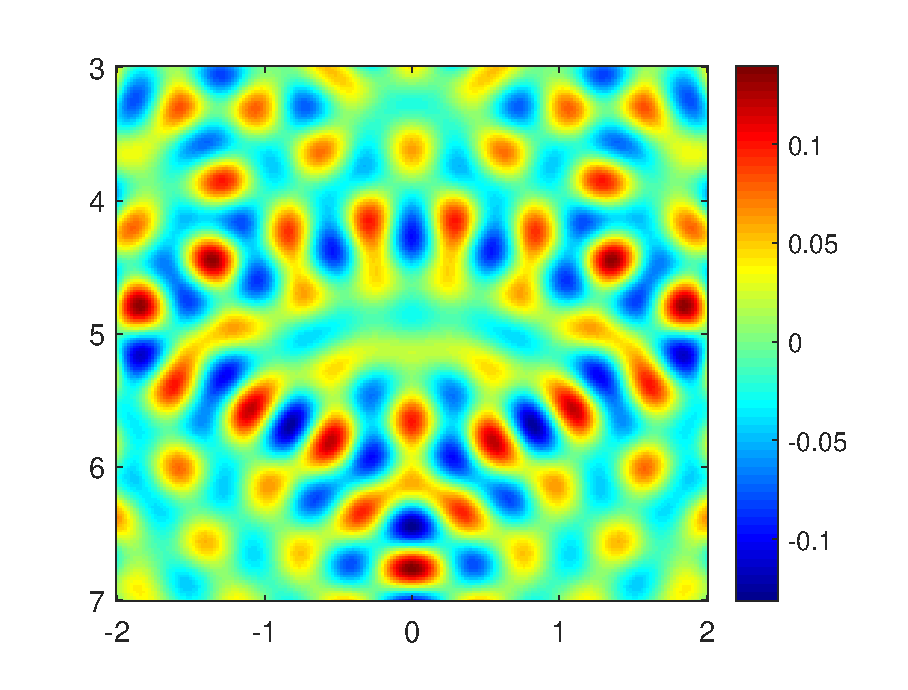
\includegraphics[width=0.4\textwidth]{./cwg/cwg_psf_real}
	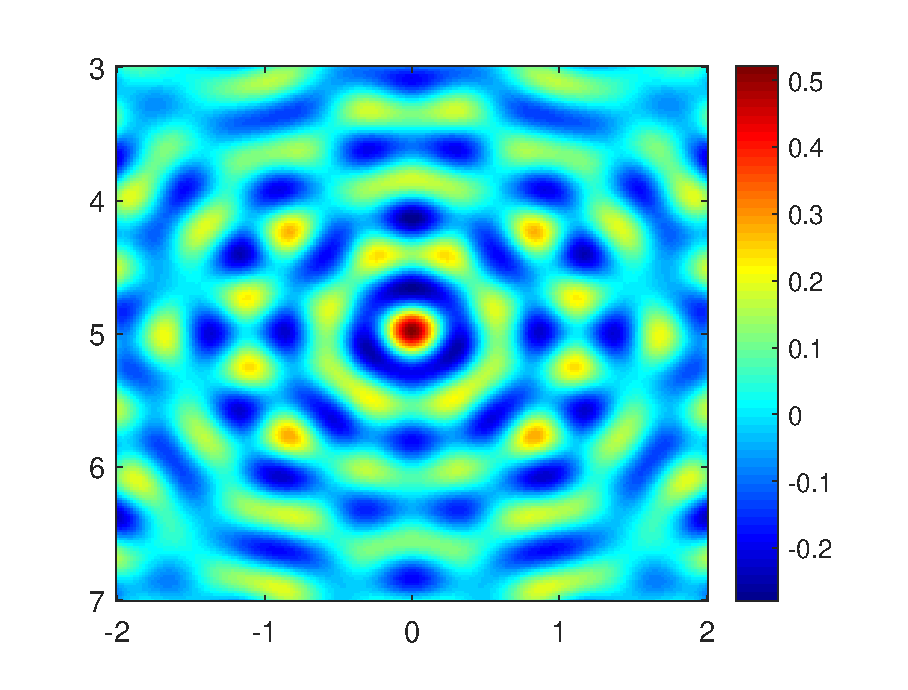
\includegraphics[width=0.4\textwidth]{./cwg/cwg_psf_imag}
	\caption{闭波导点扩散函数测试:左边为$\Re J_{w,d}(z,y)$,右边为$\Im J_{w,d}(z,y)$,其中源点$y=(0,5)$,采样区域$\Omega=[-2,2]\times[3,7]$,波数$k=12$。}
	\label{cwg_psf}
\end{figure}
由引理\ref{mode_Gw}和引理\ref{mode_Nw}可知:
\begin{equation}
 G_w(x_r,z)=G^g_w(x_r,z)+G^{rad}_w(x_r,z),\ \ 
 N_w(x_r,y)=N^g_w(x_r,y)+N^{rad}_w(x_r,y)
\end{equation}
于是有限孔穴点扩散函数$J_{w,d}(z,y)$同样可以分为如下四个部分:
\begin{equation}
 J_{w,d}(z,y)=\sum\limits_{i=1}^4J^i_{w,d}(z,y)
\end{equation}
其中
\begin{eqnarray}
\left\{
\begin{array}{lll}
 J^1_{w,d}(z,y)&=&\int_{\Gamma_h^d}\frac{\partial G_w^g(x_r,z)}{\partial x_2(x_r)}\overline{N_w^g(x_r,y)}ds(x_r)\\
 & &\\
 J^2_{w,d}(z,y)&=&\int_{\Gamma_h^d}\frac{\partial G_w^{rad}(x_r,z)}{\partial x_2(x_r)}\overline{N_w^{rad}(x_r,y)}ds(x_r)\\
 & &\\
 J^3_{w,d}(z,y)&=&\int_{\Gamma_h^d}\frac{\partial G_w^g(x_r,z)}{\partial x_2(x_r)}\overline{N_w^{rad}(x_r,y)}ds(x_r)\\
 & &\\
 J^4_{w,d}(z,y)&=&\int_{\Gamma_h^d}\frac{\partial G_w^{rad}(x_r,z)}{\partial x_2(x_r)}\overline{N_w^g(x_r,y)}ds(x_r)\\
\end{array}
\right.
\end{eqnarray}
与开波导情形类似,第一项表示波导项反传波导项,第二项表示衰减项反传衰减项,最后两项为交叉反传项。取和之前相同的参数对这四项分别进行测试,根据如图\ref{cwg_psf_part}所示的测试结果可知:与第三种开波导情形不同的是,闭波导仅有波导项反传波导项为其主要项。
\begin{figure}[t]
	\centering
	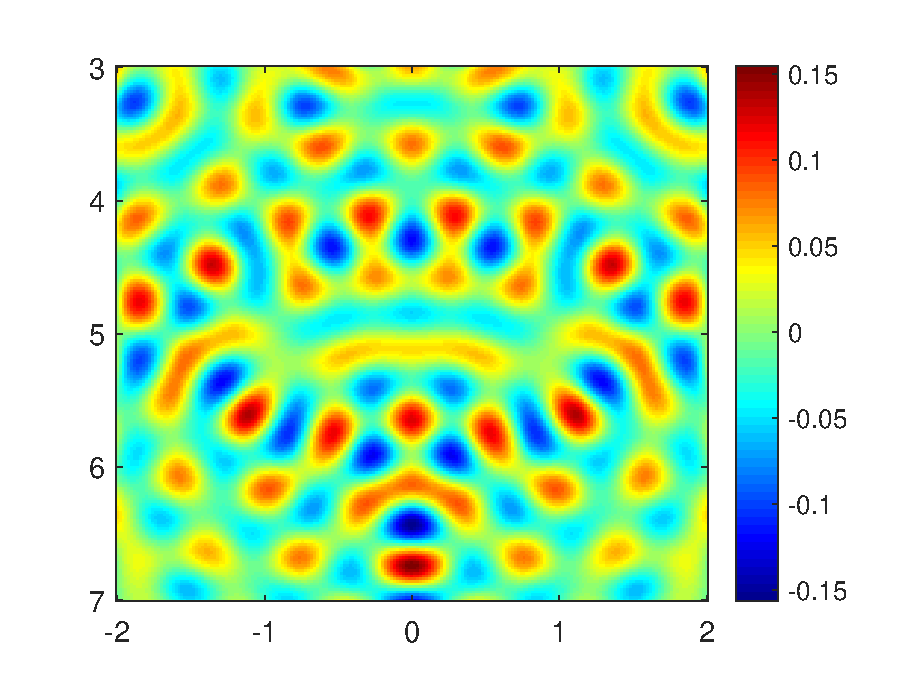
\includegraphics[width=0.23\textwidth]{./cwg/cwg_psf_real_1}
	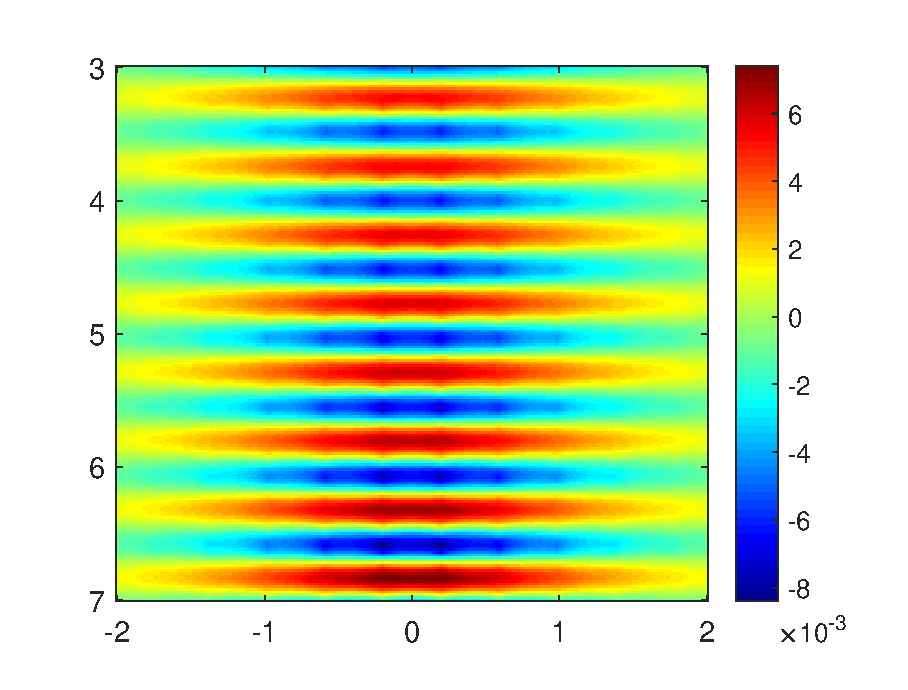
\includegraphics[width=0.23\textwidth]{./cwg/cwg_psf_real_2}
	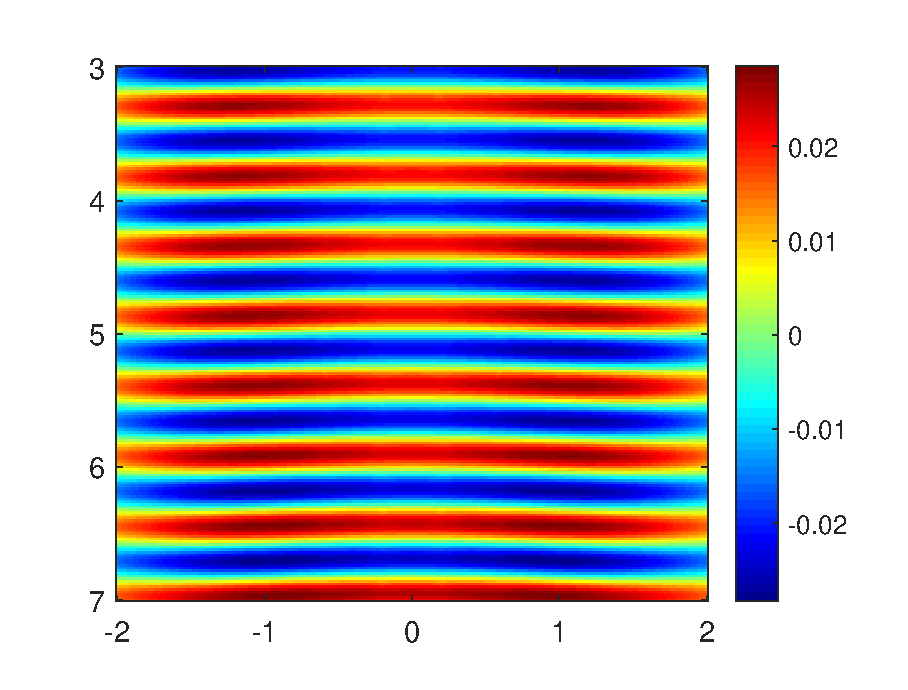
\includegraphics[width=0.23\textwidth]{./cwg/cwg_psf_real_3}
	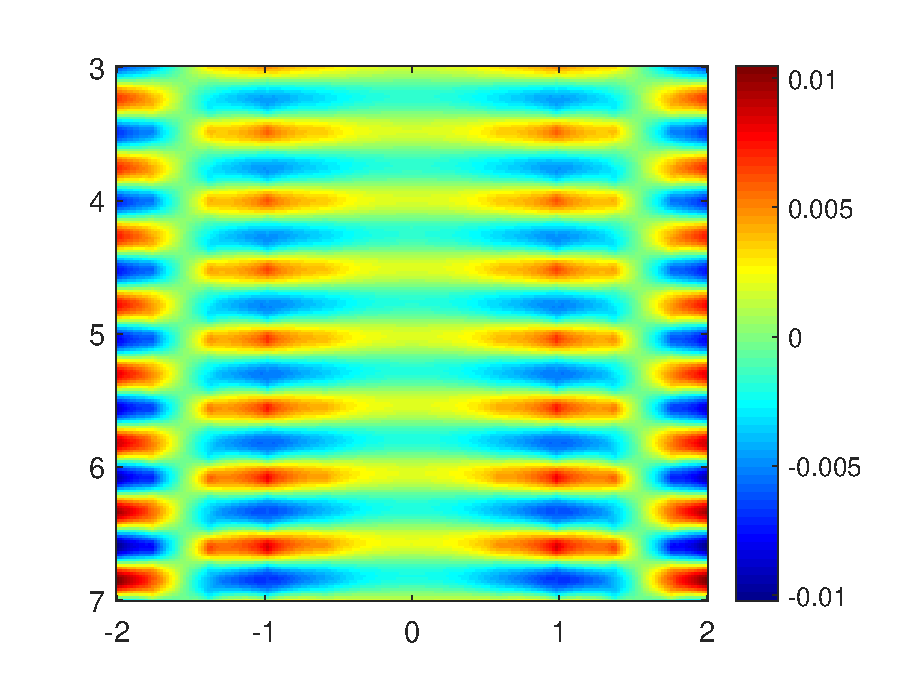
\includegraphics[width=0.23\textwidth]{./cwg/cwg_psf_real_4}
	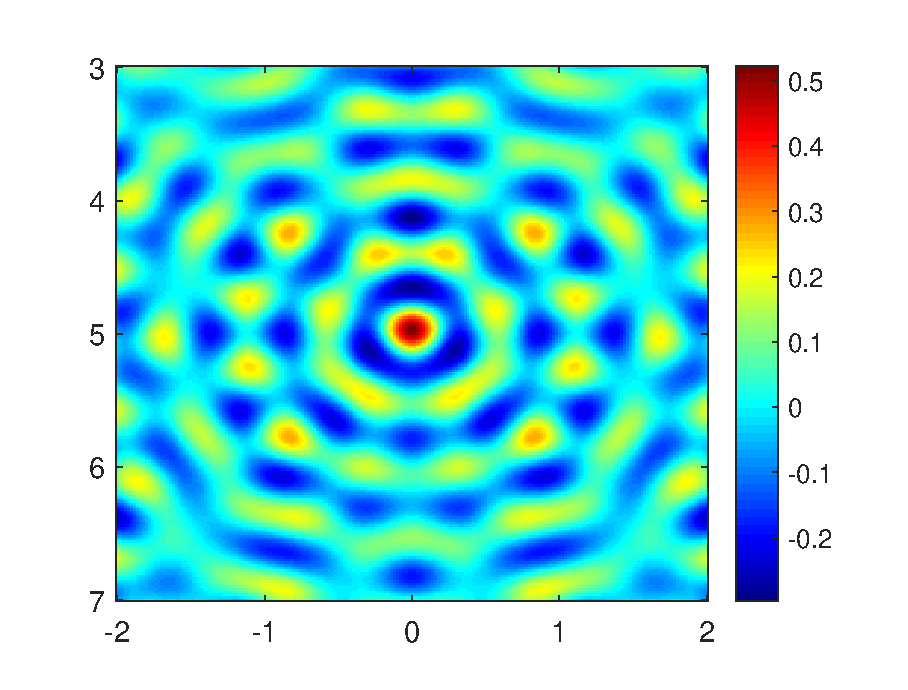
\includegraphics[width=0.23\textwidth]{./cwg/cwg_psf_imag_1}
	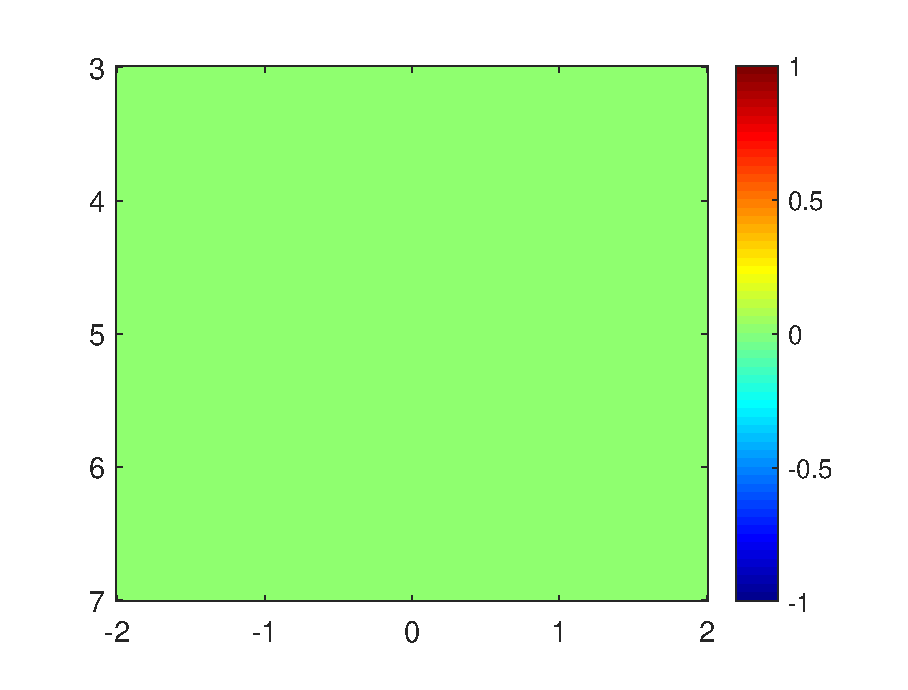
\includegraphics[width=0.23\textwidth]{./cwg/cwg_psf_imag_2}
	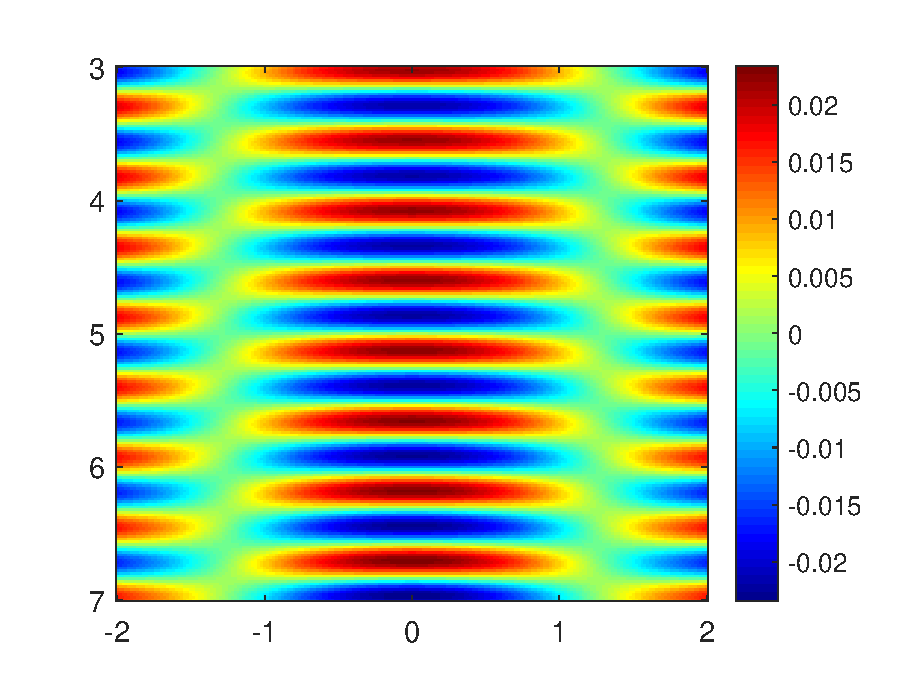
\includegraphics[width=0.23\textwidth]{./cwg/cwg_psf_imag_3}
	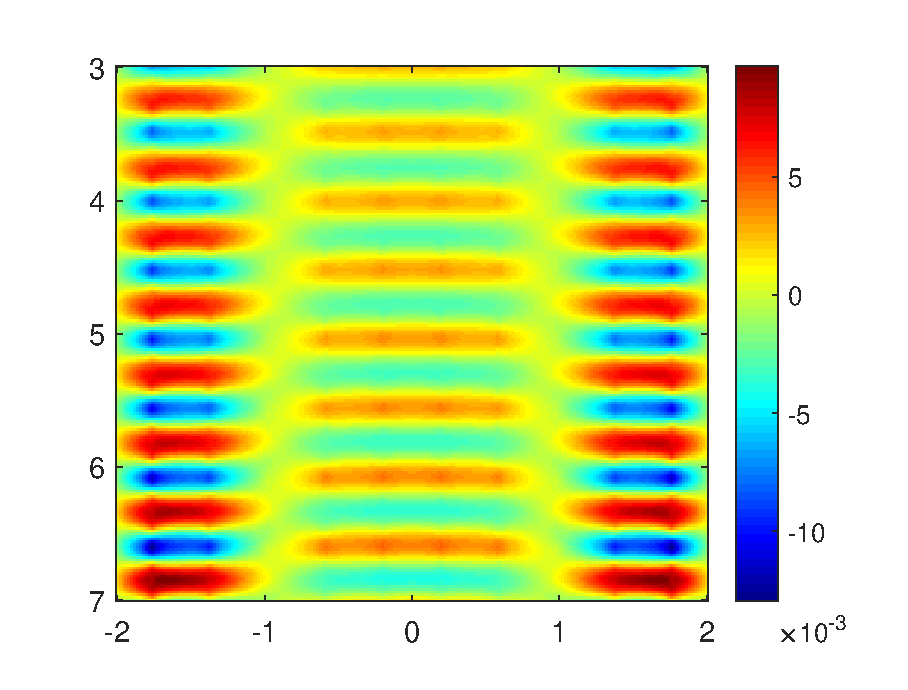
\includegraphics[width=0.23\textwidth]{./cwg/cwg_psf_imag_4}
	\caption{闭波导点扩散函数测试:从左到右依次为波导项反传波导项$J^1_{w,d}(z,y)$,衰减项反传衰减项$J^2_{w,d}(z,y)$,以及交叉反传项$J^3_{w,d}(z,y)$和$J^4_{w,d}(z,y)$,其中第一、二行分别为相应函数的实部和虚部。源点$y=(0,5)$,采样区域$\Omega=[-2,2]\times[3,7]$,波数$k=12$。}\label{cwg_psf_part}
\end{figure}
如果我们代入$G_w^g(x_r,z)$和$N_w^g(x_r,y)$的具体表达式,直接推导并化简后,则可以得到
\begin{equation}
 J^1_{w,d}=\sum\limits_{p=1}^{M}\sum\limits_{q=1}^{\hat M}f^{pq}_w(z_2,y_2)I^{pq}_d(z_1,y_1)
\end{equation}
其中函数$f^{pq}_w(z_2,y_2)$为关于$z_2,y_2$的函数,而$I^{pq}_d(z_1,y_1)$与开波导情形一样,即
\begin{equation}
I^{pq}_d(z_1,y_1) =\int_{-d}^{d}e^{\i|x_1-z_1|\xi_p-\i|x_1-y_1|\hat\xi_q}dx_1
\end{equation}
这表明在闭波导情形,我们得到了同样的结果,这是一个非常有意思的事实,下一步我们将继续对其进行研究。

\begin{remark}
	结合本章和第三章分析可知,无论是开波导还是闭波导逆时偏移算法,$I^{pq}_d(z_1,y_1)$所带来的问题均不可避免。除此之外,本文第四章中所提到的阻抗型逆时偏移算法的思想也是可以尝试解决闭波导障碍物成像问题,也就是使用函数$G_{w,\lambda}(x,y)$做为反传播函数,其中$G_{w,\lambda}(x,y)$满足如下方程:
\begin{eqnarray}\label{cwg_impedance}
\left\{
\begin{array}{lll}
\Delta_xG_{w,\lambda}(x,y)+k^2G_{w,\lambda}(x,y)=-\delta_y(x),&in&\quad \R^2_h\\
& &\\
G_{w,\lambda}(x,y)=0, &on&\Gamma_0\\
& &\\
\frac{\partial G_{w,\lambda}(x,y)}{\partial x_2}+\i\lambda G_{w,\lambda}(x,y)=0, &on&\Gamma_h
\end{array}
\right.
\end{eqnarray}
直接计算可知,$G_{w,\lambda}$的积分表达式为:
\begin{equation}
  G_{w,\lambda}(x,y)=\frac{1}{2\pi}\int_{SIP}\hat G^y_{w,\lambda}(\xi,x_2)e^{\i(x_1-y_1)\xi}d\xi
\end{equation}
其中
\begin{equation}
  G^y_{w,\lambda}(\xi,x_2)=\frac{\i}{2\mu}e^{\i\mu|x_2-y_2|}-\frac{\i}{2\mu}e^{\i\mu(x_2+y_2)}
  +\frac{\i}{2\mu}\frac{e^{2\i\mu h}}{N_{w,\lambda}(\xi)}\left[4\sin(\mu x_2)\sin(\mu y_2)\right]
\end{equation}
以及
\begin{equation}
 N_{w,\lambda}(\xi)=\frac{\lambda-\mu}{\lambda+\mu}-e^{2\i\mu h}
\end{equation}
通过测试可知,当选择合适的$\lambda$使得函数$N_{w,\lambda}(\xi)$在$\xi\in\R$上没有零点时,选择$G_{w,\lambda}(x,y)$也是可行的,有兴趣的读者可以做进一步的研究。
\end{remark}
